\documentclass[14pt]{report}
\usepackage[utf8]{inputenc}
\usepackage{blindtext}
\usepackage{amsmath}
\usepackage[margin=1in]{geometry} 
\usepackage{graphicx,changepage}
\usepackage{xcolor}
\usepackage{hyperref}
\usepackage{tcolorbox}
\usepackage{subfig}
\usepackage{fancyvrb}
\usepackage{listings}
\usepackage{svg}
\usepackage{dirtytalk}
\usepackage{csvsimple}
\newcommand\todo[1]{\textcolor{red}{#1}}
\title{Legend Of Bluespec}
\author{kr469 }
\date{October 2021}

\tcbset{colback=pink!7,colframe=pink!90,coltitle=black}
\begin{document}

\maketitle
\tableofcontents

\chapter{Introduction}

Making hardware is hard, and similarly to other problems in computer science, we make it easier by adding layers of abstraction. There are many layers involved in making hardware from that abstract transistors to gates to logical operations to functions to modules to chips to multi-chip modules to whole devices. The layer this project focuses on is going from modules to chips(TODO: this probably need renaming). At this layer we already have code for modules like memory, CPU-cores, interconnects and so on. Now what we need is an ability to compose them in such a way that they create a whole device. On a paper this should be a simple task but in reality it's a lot more complicated.

\section{Reality}
Creating custom hardware is getting more expensive both in therms of money but also in terms of man-hours needed to create it. 
This creates barriers to entry for new players, and also reinforces strong positions of already adopted standards. 
Two monoliths that I will focus on are language Verilog and design software Intel Quartus Prime(IQP). 
In my work I will work with Bluespec language that can be compiled down to Verilog. 
\begin{tcolorbox}[title=Market share and justification for focusing entirely on comparisons with Intel Quartus Prime]
    It's a bit difficult to accurately judge market share of IQP, but It is produced by one of the biggest chip manufacturer and designer in the world, and it's also used by Qualcomm according to \href{https://discovery.hgdata.com/product/intel-quartus-prime}{HG Insights}. Using Google trends tool we can see that while in recent years(since 2016) competitor Xilinx Vivado has overtaken, IQP in interest at the global scale, in most developed countries like US, Europe, and parts of Asia. There is roughly 50/50 split between IQP and Vivado. My personal observations suggest that Xilinx Vivado has been more popular in India which is a large country that is currently developing rapidly. Therefore, while I'm going to assume that IQP is still one of two biggest hardware design platforms, and it's fair to not investigate Xilinx's software during evaluation(TODO: check if this has changed).
\end{tcolorbox}
My project will try to tackle a subset of functionality provided by a tool called Platform Designer that is a part of Intel Quartus Prime package. Platform Designer is a GUI tool for connecting modules, it is capable of saving and loading designs, from proprietary plain text file format. Unfortunately, those files are not exactly what one might call "Human readable" as they have a tendency to be megabytes long(millions of characters). This tool also have some other pains that will be explained later.

\section{Solution}
During my project I will try to create an alternative file format that is much simpler and allows for editing by a human. To do this I will harness power of types in Bluespec language. My tool will be able to operate on Bluespec packages, but thanks to other tools that allow for interoperability of Bluespec and Verilog, it should be still technically possible to use my tool with wider Verilog ecosystem.

\chapter{Preparation}

\section{Understanding Bluespec}
To begin working with Bluespec we first need to understand the language.
\subsection{Rules}
 In Bluespec all computation is done in form of rules. Each cycle we will take a subset of all rules that we are going to execute in this cycle, rule is fired (executed) in cycle only if it's ready (or will be ready) and it's not conflicting with other rules (If this happens compiler must issue a warning, and picks arbitrary rule to fire from subset of conflicting rules). Each rule can fire at most one time per cycle. For rule to be ready to fire it needs it's implicit and explicit conditions to be true. Rule can be fired in a cycle even if it's not ready at the start of cycle, for example if you add item on an empty queue and then pop can happen in same cycle.\\
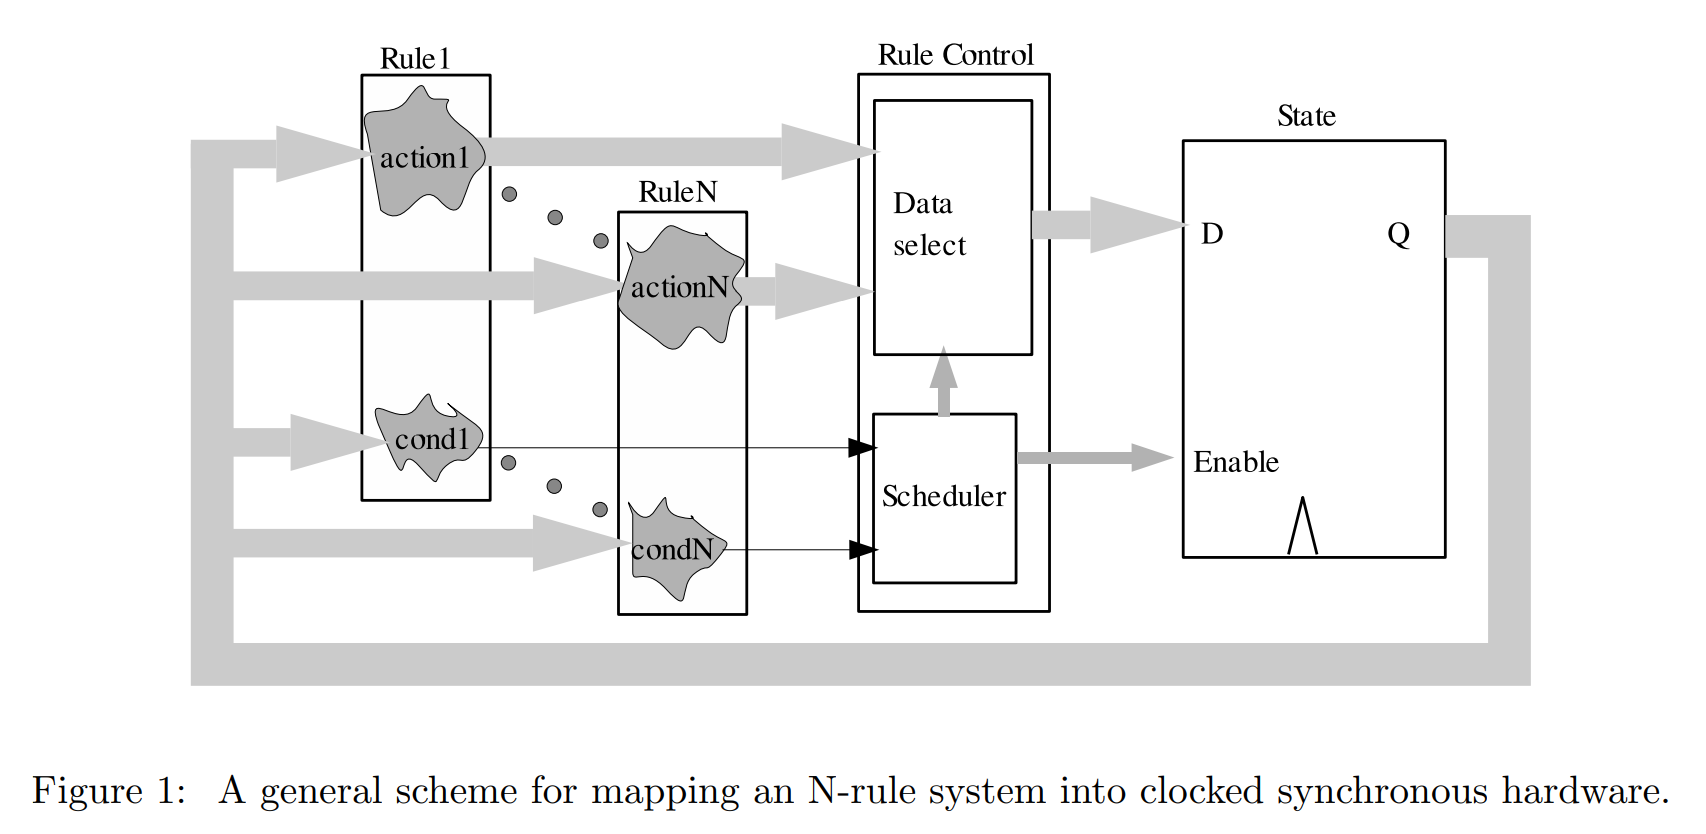
\includegraphics[width=\textwidth]{Rulemapping.png}
(TODO: add reference to the bsv reference document from which this image was taken)
\begin{verbatim}
        
    TODO: piece of Bluespec with module using fifo and other rule
     explaining types of conditions.
    
\end{verbatim}

\subsection{Modules and interfaces}
Module is something (TODO: I have no Idea how to call it). Modules don't have types, instead they implement some interface. This means that you can have multiple different modules that implement the same interface, this makes interoperability much easier. Interfaces are made up out of two things:
    \begin{itemize}
        \item Methods - that allow for interaction with the module.
        \item Subinterfaces - That allow for more generalization, for example you need to connect one more thing you don't need to change an interface used by other modules, you can just create a new interface that contains two subinterfaces and pass them accordingly.
    \end{itemize}

\subsection{Types}
Welp, there is a ton of them.
\subsection{Typeclasses}
Types classes in Bluespec are used to group types for which specific functions are implemented. TODO:

\section{Creating a grammar}

\subsection{Why grammar is needed ?}
I had effectively 3 choices for a language to write this grammar in:
\begin{itemize}
    \item Haskell - This would require me to directly tap into complier for information about modules and ect. in packages, and I would also need to learn Haskell effectively from scratch. I hope that I don't need to explain why learning Haskell while trying to understand complier of another language is a bad idea.
    \item Tcl (pronounced "tickle") - This language is used as a scripting language in both Inter and Xilinx tools, I will be reading packages using Tcl scripts provided by the creators of the Bluespec complier (BSC), but my understanding is that those scripts are just handy wrappers for some Haskell code. This is also foreign language to me with minimal presence, and negligible learning resources.
    \item Python - Firstly this is a language I have experience working with, secondly it's widely supported, and there is extensive tooling for it. It's flexible typing system allows for rapid experimenting. 
\end{itemize}
I have chosen Python for this project as I didn't want to dabble in the BSC as I was advised that this is dangerous for part II project as compliers are overwhelmingly complex and difficult to understand. This meant that I will need to parse output of Bluetcl (complier script for inspecting packages), and to do this I'm going to need grammar.

\subsection{What grammar is needed ?}
Bluetcl produces many, outputs but two of them that we are going to focus on are: descriptions of functions and descriptions of types. To simplify parsing of those I will have one grammar capable of parsing both outputs at the same time, as some grammar structures are reued in both outputs.
\subsection{Where to find this grammar ?}
Unfortunately this grammar is not documented anywhere, so I needed to reverse engineer it. This grammar might not be perfect and might not cover every input, but if created carfuly to allow for as much flexibility as possible, and use of large body of test input in from of standard library during creation of it we should be exposed to enough examples to be able to parse decently large subset of future inputs.
Here are other reasons to justify this approach:
\begin{itemize}
    \item Heaps' law suggests that number of unique words in given body of text is proportional to roughly square root of number of words in the text. I think it's fair to assume that something similar will be true if we consider number of unique grammar rules.
    \item This grammar while different from grammar of Bluespec language maps subset of Bluespec grammar, so we can supplement our deductions with cases that we expect to arise.
    \item We don't need to understand everything to just connect modules, and because at the module level, things need to be less abstract as they need to be synthesizable, we don't expect highly exotic things to appear in higher level modules.
    \item This approach is probably the best way for me anyway.
\end{itemize}

\subsection{Technical aspects}
This is EBNF grammar, I parse it using Lark library for Python, and I'm using Earley parser, as it is capable of arbitrary length lookahead. Grammar I created contains roughly 90 rules, and I won't include all of them here, but I will show few examples to give a feel of what is happening.
\begin{tcolorbox}[title = Parsing position TODO maybe find a better example with shorter line]
    \begin{verbatim}
tcl_position: "{" "position" "{" tcl_path NUMBER NUMBER ["{" "Library" identifier_u "}" ]"}""}"
// todo check paths with spaces
tcl_path: ["%/"] /(([.]{1,2})|(\w+))/ ["/" /(([.][.])|([.])|(\w+))/]* "." /\w+/

-------- Text to parse ---------
{position {%/Libraries/Connectable.bs 25 1 {Library Connectable}}}
    \end{verbatim}
    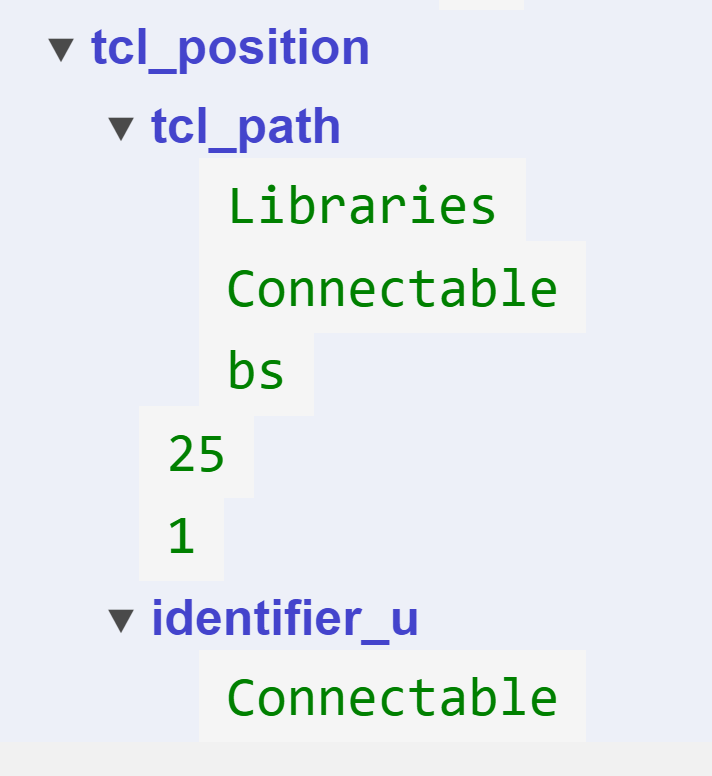
\includegraphics[width=0.4\textwidth]{images/TCLPath.png}
\end{tcolorbox}
A nice feature supported by Lark is ability to have regular expressions in the grammar, I'm mentioning this as is effectively having parser in side of parser. A handy tool for debuging and creating grammar was this website: \href{https://www.lark-parser.org/ide/}{https://www.lark-parser.org/ide/}, it can run parser online, and show output tree.

\chapter{Implementation}
\section{Reading packages}
\subsection{Bluetcl}
As mentioned before, bluetcl is a tool written in bash that starts Tcl terminal and sets up environment to use certain Tcl commands thanks to which one can inspect packages. To interact with this tool I have written a script using Pexpect library. This script works by creating subprocess of bluetcl, and exposes functions that allow for performing quarries. Core of this script is a function called \verb!call! that takes as input a string that is a command and returns output of stripped of warnings or raises an exception if error occurred(for example in case where package was not found). To remove warnings I make some assumptions.
\begin{itemize}
    \item I only use fixed set of commands.
    \item For those commands important output about is always on the last line. (this was checked empirically)
    \item Output of a command is always followed by $\%$ a character that never occurs in the rest of the output and marks the end of the output.
\end{itemize}
Thanks to them I don't need sophisticated system for parsing error, and or warnings. I can just make a quick search for error, and if needed forward this to user otherwise drop all warnings.
\\ 
\\
In total this script allows me for:
\begin{itemize}
    \item Initialize subprocess
    \item Add folder to search path of bluetcl
    \item Load package (bluetcl takes care of loading dependencies)
    \item Get list of loaded packages
    \item List functions in package
    \item List types in package
    \item Get information about types and function in the package
\end{itemize}

\section{Parsing}
Output of bluetcl is text, and I need it in some better organized form, so I can parse it. I decided to use Lark library for parsing, and I'm using Earley parser. At this step I encountered first major difficulty that is total lack of documentation on form bluetcl output. I decided to reverse engineer it, and I'm using this website: \href{https://www.lark-parser.org/ide/}{https://www.lark-parser.org/ide/} to debug and create grammar, it can run parser online, and show output tree. To aid myself in this process I consulted Bluespec reference guide. While bluetcl output was undocumented it still needed to map to features of Bluespec. In total, I produced grammar with roughly 80 non-terminals.

\subsection{Understanding abstract syntax tree (AST)}
Given AST I needed to turn it into a more useful form. To do this I used \verb!Transformer! class provided by Lark. The way it worked is that I created subclass of \verb!Transformer! that implemented a function for each non-terminal / rule(Each non-terminal can have multiple rules and Lark allows for renaming individual of rules, this for example allows parsing different non-terminals using same function or parsing single non-terminal using different function depending on constructing rule). \verb!Transformer! will then perform bottom up transformation of AST, and for each rule it will call respective member function, with parsed children as arguments. At the end of the transforming process I would have a list of objects that represented data from Blutecl.
\\
One of the bigger inconveniences I encounter is the fact that Lark passes parsed children, as a simple list. This doesn't provide information about what exactly is each child, this isn't a problem if rule contains fixed number of non-terminals, but otherwise I employ mix of length based inference, or I wrap data from children into tuples, to provide remove ambiguity.
\\
What was quite useful at this stage is Python's type system flexibility, I was able to gradually build up system and add typing information only after I had firm understand what type something needs to be. For some things it wasn't imminently obvious, what is the best way to represent type, and what often happen is that I would shape type to needs of the functions using it and not other way. 

\subsection{Organizing data and functionality}
I created a class called \verb!TypeDatabase! it is basically a wrapper over previously mentioned functionality that manages organizing parsed output into separate dictionaries, like types, functions, type classes ect. It is also capable of loading and storing it's state to pickle file. This saves a lot of time as all this parsing and communication with bluetcl isn't particularly fast. TODO some break down of the speed.

\section{Building the top level module}
Building the top level module can be broken down into few operations.
\begin{itemize}
    \item Instantiating new modules.
    \item Connecting modules using \verb!mkConnection! function.
    \item Connecting modules using busses.
    \item Synthesizing Bluespec.
\end{itemize} 
Those operations if implemented naively would be almost as simple as formatting a string. But If this was the only thing that this project provided I wouldn't need to go through all the trouble of parsing Bluespec grammar, and generally users would be better off just writing Bluespec code. My unique proposition is effectively running something similar to a language server, that will be capable of dynamically resolving types, and aiding user in the design process by providing possible connections, informing whether values passed to initialize module are correct, and informing about subinterfaces that can be found in the instantiated modules. 
At the basis of all those features will be type resolution, and to do it we first need to talk about do we do this.
\subsection{Resolving types}
\subsection{Provisos explained (intuition)}
On big feature of Bluespec typing is support for provisos. They create constraints on types that can be used with given function and give information about expected type of output of the function. This is similar to how C++ has template types, but it is much more powerful. For example, we can have a polymorphic function from \verb!Bit#(a)! to \verb!Bit#(b)! and $a=b+1$ where \verb!Bit#(x)! a vector of $x$ bits.  To do something like this we would write a proviso \verb!Add#(b,1,a)! which means that $b+1$ must be equal to $a$.
\\
System of provisos and typeclass work similarly to Prolog. We have variables that are lowercase names, we have values that are either strings or integers, and we have parametric types that are like compound terms. Typeclass instances are like rules and provisos attached to it are like predicates. To resolve types I do something I run Prolog style resolution. 

\subsubsection*{Provisos explained (formally)}
There are two types of provisos: Size Relationship provisos, and typeclass based provisos.

Mentioned above \verb!Add! is one of Size Relationship provisos, other such provisos are \verb!Mul Div Max Min Log!. Those provisos can't be nested, but we still can express complex arithmetic constraints, thanks to size relationship type functions. They essentially represent result of the operation on values on that were supplied. There are only 8 of them, and they are \verb!TAdd TSub TDiv TMul TMax TMin TLog TExp!.
To better explain this let's look at some simple example: \\
\verb!Add#(TExp#(a),TMul#(a,8),c)! is a proviso that says that following equation on values must be satisfied $2^a+a*8 = c$. \\
Of course, we can have multiple provisos that together create a set of equations. 

Typeclass based provisos, allow us to either check if certain functions are defined for given type or to deuce something. For example \verb!Bits#(a,b)! means that type \verb!a! must be convertible to vector of $b$ bits. This can be used to get the length in bits of given objects, on which we can later put constraints using Size Relationship provisos.
In my project I will often check if there exists instance of the \verb!Connectable#(a,b)! typeclass to check if function \verb!mkConnection!(used to connect two interfaces together) is defined for given types.

\subsection{Resolving types (implementation)}
In my code there are 4 main functions that combined allow for type resolution:
\begin{itemize}
    \item \verb!merge! function takes two type identifiers and returns dictionary from names of variables to theirs values.
    \item \verb!applyVariables! function takes a dictionary and a type and returns a type with all variables replaced by their values.
    \item \verb!resolveTypeclass! function that takes a type identifiers that is an instance of a typeclass and returns dictionary similarly to merge.
    \item \verb!solveProvisos! function that takes a dictionary and a list of provisos and returns a dictionary with all provisos resolved.
\end{itemize}
Those functions can also fail with exception if something is impossible.

Type identifier is a tree where every non leaf node is another type identifier, and leaf nodes are either variables or values(strings, ints). Example type identifier \verb!Foo#(a,42,"file.hex")! is a type with name \verb!Foo! and three arguments \verb!a! (variable) and \verb!42! (int value) and \verb!"file.hex"! (string value).

\subsubsection*{Merge function}
This function works like a two synchronized dfs's, that go through the trees (type identifiers) and apply logic based on nodes that are beginning currently visited.
This function needs to account for quite a lot of special cases here are some of them:
\begin{itemize}
    \item If one of the nodes is a variable, and other is a value or another type identifier, then we can add such pair to the dictionary of resolved variables.
    \item If both nodes, are type identifiers, we run merge recursively on pairs of theirs children. We also check if type identifiers share the same name.
    \item If one of the nodes is a value, then other node must be either a value with same value, or a variable.
\end{itemize}
The most complicated case is when both nodes are variables, this is because we need to account for the case where both variables have a value and check if this value is equal. If only one of them has value and this value needs to be copied to other one, or if neither of them has value, then we we must create dummy object and set it as a value of both of them, then if one of them is resolved it will such resolution will resolve other one, by virtue of shared pointer.

\subsubsection*{Apply variables function}
This function is quite simple, it just traverses a type identifier and replaces all variables with their values.
\subsubsection*{Resolve typeclass function}
Earlier, I compared typeclass to groups of Prolog rules, one thing I didn't mention that typeclasses can also contain something called dependencies, they are something like marking inputs and outputs in Prolog. Those dependencies are used for typeclasses like \verb!Bits#(a,b)! that are used to determine something, and they make are there to use of typeclass is always unambiguous. \\
For example, \verb!Bits#(a,b)! has a dependency \verb!a determines b! which means that you can use it to determine \verb!b! from \verb!a!, but if you know only \verb!b! then you can't use it to determine \verb!a! because there may be multiple types that can be packed to a bit vector of length \verb!b!. 
\\  
To check if proposed instance of a typeclass is a valid instance we perform following algorithm:
\begin{enumerate}
    \item Check if a proposed instance of a typeclass is an instance of a known typeclass, otherwise fail.
    \item Check if all dependencies of the typeclass are satisfied, otherwise fail.
    \item Iterate over all known templates of an instance of a typeclass, then attempt to merge function between a template and the proposed instance. 
    \item If merging failed, jump back to step 3 and continue iteration.
    \item If merging succeeded, attempt to solve provisos.
    \item If provisos were successfully solved, return the dictionary of resolved variables, otherwise continue iteration.
    \item If all iterations failed, fail.
\end{enumerate}
This procedure is a bit slow, so I also allow a passing of an suggested list of instances of a typeclass, which will be iterated over. In specific scenarios like, when user creates connection between two interfaces, I can run a heuristic that only checks if names of type identifiers match, to quickly trim search space. Doing this in general is non-trivial, due to existence of dependencies. As it's possible to have typeclass like this:
\\
\verb!Foo#(a,b,c)! where \verb!a determines b,c! and \verb!b,c determines a! then I would need to check which case this is then to do lookup in a dictionary corresponding to that dependency. Preprocessing of such dictionaries would take something like $O(nInstances^2*nDependencies)$ time, and it would add unnecessary complexity. (Though it's something that might be worth looking in the future.)

\subsubsection*{Solve provisos function}
TODO (I think my implementation is bugged as it can fail, in an edge case due to ordering of provisos)

\subsubsection*{How those functions can be used}
Thanks to those functions, my code can check if types of arguments given by the user are correct (thanks to merge function). I can check if enough information about expected resulting type of overloaded function was given and if so, I can use it to deduce types of subinterfaces.

\section{Synthesizing}
The goal of the project is to be able to take a JSON with some data and synthesize a top module in the Bluespec language from it. This goal is more like a justification to create a language server like API. With this approach I have some simple core goal, but in the later sections we will see how thanks to all the work I can use this API to support GUI that aids the user in creating a top module. Therefore, I will focus in this section on how the API works, and only later how is it used when reading JSON or as a backend to the GUI based app.

\subsubsection*{Top level module object}
Let's start with quick overview of the functions found in API.
\begin{itemize}
    \item \verb!addModule! as the name suggest this function adds an instance of a module.
    \item \verb!addConnection! Essentially a wrapper on a \verb!addModule! function that adds connection between two interfaces.
    \item \verb!addBus! given list of slaves and masters it adds a bus with those interfaces connected.
    \item \verb!listConnectable! is a function not meant to be called directly by the user, it will be called by the \verb!addModule!, and it will populate the dictionary of possible connections (that user can use).
    \item \verb!remove! to remove previously added things.
    \item \verb!to_string! that returns a string representing \verb!.bsv! file with top module as defined by previous calls.
\end{itemize}

\subsubsection*{Adding modules (introduction)}
Adding an instance of a module in Bluespec is done by calling function used to instantiatie chosen module, and potentially assigning it to a variable of a type of interface produced by a function. It's worth keeping in mind that not all such functions can create new modules (those who do are called modules and one that don't are called functions in Bluespec), for example \verb!fromAXI4LiteToAXI4_Master! is a function that will take already existing instance with \verb!AXI4_Master! interface and return \verb!AXI4Lite_Master! interface, and all of this will be done by just assigning functions and subinterfaces found in one to the other one. Fortunately, there is no need for me to treat modules different from the functions. The only thing that will be treated differently are busses and connections, as they are functions like described above but theirs result interface is \verb!Empty!(similar to void in C++), so there is no need to assign them to a variable.
\\
One more decision I had to make was whether I want to support \verb!let! as a type. \verb!let! keyword is used to omit writing type of variable explicitly. This makes it so compiler has to deduce it from the output of a function defining such variable. While Bluespec is strongly typed language it's not always possible to use \verb!let!. For example, in cases where you create a module with polymorphic interface, there might not be enough information to deduce the full type of the interface. What's even more confusing is that sometimes you only need to provide some subset of variables in the type of interface, and the rest can be deduced using provisos. (TODO check this) Bluespec doesn't support something like this, but I do. On the other hand I don't support \verb!let! keyword and I will always write out full type explicitly, this makes it harder to modify the code, as some changes might require more changes down the line, but this produces more readable code, also making such changes is still quick if done before code generation.
\subsubsection*{Adding modules (implementation)}
Here is a procedure of instantiating a module:
\begin{enumerate}
    \item Check if name string is a valid name and starts with lowercase.
    \item Create an instance object.
    \item Call update function of that object, that will verify correctness of the arguments and it will update global state. In more detail update function does following:
    \begin{enumerate}
        \item Parse user given strings that represent arguments. This includes 
        \item Run a unification (merge function described earlier) to check if types of arguments are correct.
        \item Run a unification on between user defined resulting type of interface and the type of interface given by the function. This produces set of context variables.
        \item Attempt to solve provisos attached to the function, with the context variables, and populate the context with newly learned variables.
        \item Apply variables to the type of interface, filling out unknows.
        \item Populate type of the instance with member subinterfaces.
        \item Add interface, and it's member subinterfaces to a global dictionary of accessible names. During this addition we also propagate updates, if for example 
    \end{enumerate}
\end{enumerate}

\subsubsection*{Adding connections}
With creating instances explained above, adding connections become trivial. We just create and instance of \verb!mkConnection! and ad it into list of known connections if we ever need to remove it.

\subsubsection{Adding busses}
Similarly to adding conenctions a lot of complexity is handled by logic to create instances, as bus is just a function that takes vectors of masters and slaves and routing function that specifies how addresses map to slaves. Two differences from standard instance is automatically instantiating of a vector that hold masters and slaves and generating routing function. \\
Instantiating of vectors was a bit tricky due to two conflicting requirements:
\begin{enumerate}
    \item I wanted to give user an option to create a vector on their own, and if elements of such vector are updated, I wanted to propagate the update to all instances using that vector.
    \item I wanted to create a vector automatically when creating a bus, so users don't have to create it manually.
\end{enumerate} 
This created a feedback loop, where update of a bus caused update of vectors used by this bus, and so on. To fix this I moved the updates of vectors to initialization of a bus, and allow for updates of vectors that are "silent" and don't cause updates. 
\\
Routing function is a function that takes a route and produces one hot vector, that specifies which slave is used for a given address. 
To create a routing function two things must be created. First I need to create a new function to be added to the database of known functions. To do this I just reuse my parsing tooling. As for creating code for it, I generate it by simply adding \verb!if! statement for each address region. I also generate comments giving information about which slave occupy which address region.

\subsection*{JSON interface}
I decided that my \say{human-readable format} will be JSON. This is because wide support for JSON is already available in many languages. The only problem of JSON is that it's more verbose than Bluespec, and in theory it would make more sense to use Bluespec. However, this could introduce user confusion, as I wouldn't be able to support arbitrary Bluespec features. My understanding is that supporting something only partially could lead users to think that my tool is broken, because it doesn't match theirs assumptions about what it can do. While it can be argued that if I had written this project as extension of Bluespec compiler I could have supported all features of Bluespec (thanks to already written logic). As explained at the beginning of this document, doing this was infeasible for me as a part II project. \\
With this out of the way let's talk about how I'm using JSON files.
\subsubsection*{Structure of JSON file}
At the top level of the file user can define following things:(TODO change those names to something more descriptive)
\begin{itemize}
    \item \say{additional folders} - This should be a list of folders that will be added to Bluespec's search path used to find modules.
    \item \say{packages} - List of packages that will be loaded. Theirs dependencies will be loaded automatically.
    \item \say{name} - Name of the top module.
    \item \say{packageName} - Name of the package, and therefore the file that contains the top module.
    \item \say{typedefs} - List of typedefs that will be added to the global scope. \\
    \begin{itemize}
        \item \say{name} - Name of the typedef.
        \item \say{value} - Value of the typedef.
    \end{itemize}
    \item \say{modules} - List of modules that will be created. \\
    \begin{itemize}
        \item \say{name} - Name of the module.
        \item \say{function} - Name of the function that will be used to instantiate the module.
        \item \say{function\_params} - List of parameters that will be passed to the function. (optional if function dose not take any parameters)
        \item \say{interface\_params} - List of the parameters of created interface. (optional if it's possible to deduce them from functions type)
        \item \say{context} - TODO implement, ability to pass only specific interface parameters
    \end{itemize}
    \item \say{connections} - List of connections that will be added to the global scope. \\
    \begin{itemize}
        \item \say{from} - Name used to access interface on the left side of the connection.
        \item \say{to} - Name used to access interface on the right side of the connection.
    \end{itemize}
    \item  \say{busses} - List of busses that will be added to the global scope. \\
    \begin{itemize}
        \item \say{name} - Name of the bus. (optional)
        \item \say{function} - Name of the function that will be used to instantiate the bus.
        \item \say{masters} - List of names used to access interfaces that will be used as masters.
        \item \say{slaves} - List of slaves. \\
        \begin{itemize}
            \item \say{name} - Name used to access the interface.
            \item \say{routes} - List of lists length two that specify starts and ends of address regions that will be used by this slave. \\
        \end{itemize}
    \end{itemize}
\end{itemize}

\subsubsection*{Using JSON interface}
At this point if all I did was simply synthesizing a Bluespec file from JSON, it would be possible to do that just by doing simple string manipulation. I know this because my initial iterations were doing this. However, my tool can do more than that, the important feature is this tools ability to display all possible connections' user can make between interfaces and subinterfaces. It is also able to show what possible valid master and slaves are for a given bus(Assuming at least one master and slave are present as otherwise it doesn't make sense). Finally, it can also display types of all interfaces and subinterfaces. This can be useful when using complex modules, like a core that doesn't have any direct connections, but It has many subinterfaces that can be connected to things like memory, external devices, etc. \\

\subsection{GUI}
Adding GUI was an optional goal mentioned in the project proposal. I originally intended to use some game engine to create a GUI, but Bluespec compiler is a Linux tool and game engines like Unreal Engine 4 or Unity3d are meant to be used on Windows, I decided against that idea. Instead, I found a library called React Flow, that provided nice API for creating graph based user interfaces. After some though I decided to create a GUI as a website. This was quite an adventure as It was my first contact with full stack web development. (I have done backend in .NET and \verb!C#! for group project in last term, but it was mostly focused on writing queries to database)


\subsubsection*{Backend}
For backend, I had a choice between Django and Flask. After reading about them in theory Flask was supposed to be better for small projects, like this one. However, I decided to use Django because I wanted to learn technology that might be more useful in the future. I followed official tutorial on Django and after initial pain with security adding functionality was easy.

\subsubsection*{Frontend (React)}
Frontend was written in React.js as you might have guessed from the name of the library I wanted to use. According to \href{https://insights.stackoverflow.com/survey/2021#most-popular-technologies-webframe}{Stack Overflow 2021 survey} React.js is the most popular frontend technology in 2021, so again I considered time spent on learning it to be good investment. One thing that took me quite a bit to get used to is everything being a function(React.js supports classes, but it's an old paradigm and I wanted to learn doing thing the \say{correct} way). This makes working with variables a bit tricky, as changes to state variable cause re-rendering of the whole component, and if variable is not a state variable, then it's value is going to be lost after re-rendering. If not careful is easy to cause feedback loop causing infinite re-rendering and subsequent crash of the application. 

\subsubsection*{Frontend (React Flow)}
\begin{tcolorbox}[title=Vocabulary]
    \begin{itemize}
        \item Handle - Is a component of node that is used to start or end a connection. TODO include a image of a handle.
    \end{itemize}
\end{tcolorbox}
React Flow from developer perspective requires defining nodes (they can be basically and arbitrary React components), and some metadata about displaying a graph that is things like how edges look, how user can add new nodes, etc. 
The exposed API is quite simplistic. 
For example position of a handle is constrained to the middle of side of a node, and this library will generate CSS to put it there. 
Therefore, I needed to write some finicky CSS to align handle with text displaying its name. [TODO improve this sentence.]
\\
Another thing that is problematic about React Flow is that it will cause node component to update every time it is moved. 
What I found is that if you wrap larger subcomponents of a node in \verb!memo! from React, then performance stays quite good even if multiple nodes are moving.   
\\
On the bright side after I figured out workarounds for those issues, I was left with many other things being handled by library. This included automatic graph formatting, and pretty Bézier curves for edges. 

\subsubsection*{Frontend (MUI)}
My default HTML buttons, and text boxes are ugly. So I decided to use React UI component library called MUI (previously Material UI). I don't have much to say about it except that use of it was seamless, at least in my humble option made my application look modern. I'm mentioning this as one of my complaints about Intel's QSys was that it's UI is decades old.

\end{document}
